\section{Čo je dualita}

\noindent
V predchádzajúcich častiach sme sa snažili ukázať, že lineárne programovanie je
silný a flexibilný nástroj pre riešenie optimalizačných problémov. Teraz sa zoznámime s ďalšou 
jeho podstatnou vlastnosťou, ktorá sa bude dať tiež mnohostranne využiť pri návrhu
algoritmov. Tou vlastnosťou je tzv. {\em dualita}. 
Predpokladajme, že Róbert chce  nájsť minimum funkcie 
$$f(x_1,x_2,x_3):=10x_1+3x_2+5x_3$$ 
spomedzi takých hodnôt $x_1, x_2, x_3$, ktoré sp\'lňajú
\begin{eqnarray}
\label{LP_001}6x_1 + \phantom{2}x_2 - \phantom{3}x_3&\ge&2\\
\label{LP_002}2x_1 + 2x_2 + 6x_3&\ge&8\\
6x_1 + 3x_2 + 5x_3&=&30\nonumber\\
x_1,x_2,x_3&\ge&0\nonumber
\end{eqnarray}
Angela vidí, že je to lineárny program a ľahko nájde minimum. Otázka je, ako má 
o tom presvedčiť Róberta, ktorý lineárne programovanie nepozná. 
O hornom odhade ho presvedčí ľahko: ukáže mu ako {\em svedka} nejaké konkrétne riešenie. Angela môže
napríklad vybrať vektor $x_1=2$, $x_2=6$, $x_3=0$ a Róbert z toho ľahko zistí, že hľadané minimum
je nanajvýš $38$. Ako ale nájsť svedka pre odhad z opačnej strany? Angela môže napríklad skúsiť 
takýto argument: ''{\em Pozrime sa na riadok (\ref{LP_001}). Akékoľvek nezáporné čísla $x_1$,
  $x_2$, $x_3$ zvolíme, vždy bude platiť $6x_1\le10x_1$, $x_2\le3x_2$ a $-x_3\le5x_3$. Preto
  $6x_1+x_2-x_3\le f(x_1,x_2,x_3)$. Lenže podľa  (\ref{LP_001}) je $6x_1+x_2-x3\ge2$,
takže každá prípustná hodnota (a teda aj minimum) funkcie $f$ je aspoň 2}''.
Angela môže pokračovať napríklad tak, že sčíta riadky (\ref{LP_001}) a (\ref{LP_002})
a použije rovnaký argument. Môže aj každý riadok prenásobiť nejakým číslom (v 
riadkoch (\ref{LP_001}) a (\ref{LP_002})
to musí byť nezáporné číslo) a sčítať ich dokopy; ak platí, že výsledná lineárna kombinácia
ľavých strán obmedzení 
je po zložkách menšia ako funkcia $f$, lineárna kombinácia pravých strán tvorí dolný odhad minima.
Aby poskytla čo najlepší argument, Angela vlastne rieši lineárny program:
nájsť maximum funkcie
$$g(y_1,y_2,y_3):=2 y_1+8 y_2+30 y_3$$
spomedzi takých hodnôt $y_1, y_2, y_3$, ktoré sp\'lňajú
\begin{eqnarray*}
6y_1 + 2y_2 + 6y_3 &\le& 10\\
y_1 + 2y_2 + 3y_3 &\le& 3\\
-y_1 + 6y_2 + 5y_3 &\le& 5\\
y_1,y_2 &\ge& 0
\end{eqnarray*}
V tomto prípade je na jednej strane svedok $x_1=0$, $x_2=5$, $x_3=3$, že hľadané minimum $f$ je najviac 30,
na druhej strane svedok $y_1=y_2=0$, $y_3=1$ ukazuje, že 30 je skutočná minimálna hodnota $f$.
Je to náhoda, že sa podarilo touto metódou nájsť tesný odhad?

\noindent
Pozrime sa všeobecnejšie na to, čo sa dialo. Majme nasledovný lineárny program, ktorý nazveme {\em primárny}
$$
\begin{array}{rrrrrcl}
  {\rm minimalizovať}     & c_1x_1     & + c_2x_2       & + \cdots  & +c_nx_n  \\
  {\rm pri\ obmedzeniach} & a_{1,1}x_1 & + a_{1,2}x_2   & + \cdots  & +a_{1,n}x_n  & \ge & b_1 \\
                          & a_{2,1}x_1 & + a_{2,2}x_2   & + \cdots  & +a_{2,n}x_n  & \ge & b_2 \\
                          &   \vdots   &   \vdots       &   \ddots   &  \vdots      &  \vdots & \vdots\\ 
                          & a_{m,1}x_1 & + a_{m,2}x_2   & + \cdots  & +a_{m,n}x_n  & \ge & b_m \\
                          &\multicolumn{4}{r}{x_1,\ldots,x_n}&\ge&0
\end{array}
$$
alebo skrátene
$$ (P): \min_{\bm{x}\in\R^n}\left\{ \bm{c}\tr\bm{x} \mid A\bm{x}\ge\bm{b},\;\bm{x}\ge\bm{0}\right\}.$$

\noindent
Dolný odhad minima $(P)$ hľadáme ako vhodnú lineárnu kombináciu obmedzení: $j$-te obmedzenie 
prenásobíme na oboch stranách koeficientom $y_j\ge 0$ a sčítame.
Chceme nájsť koeficienty $y_j$ tak, aby ľavá strana bola menšia ako minimalizovaná funkcia 
$$ \sum\limits_{i=1}^nc_ix_i\ge \sum\limits_{j=1}^m y_j 
\left(a_{j,1}x_1 + a_{j,2}x_2 + \cdots + a_{j,n}x_n\right) \ge  \sum\limits_{j=1}^my_j\cdot b_j. $$

Keďže $x_i\ge0$, prvá nerovnosť platí, ak platia nerovnosti v koeficientoch pri každom $x_i$. Najlepší
dolný odhad, aký touto metódou môžeme získať, je preto riešením
{\em duálneho} lineárneho programu
$$
\begin{array}{rrrrrcl}
  {\rm maximalizovať}     & b_1y_1     & + b_2y_2       & + \cdots  & +b_my_m  \\
  {\rm pri\ obmedzeniach} & a_{1,1}y_1 & + a_{2,1}y_2   & + \cdots  & +a_{m,1}y_m  & \le & c_1 \\
                          & a_{1,2}y_1 & + a_{2,2}y_2   & + \cdots  & +a_{m,2}y_m  & \le & c_2 \\
                          &   \vdots   &   \vdots       &   \ddots   &  \vdots      &  \vdots & \vdots\\ 
                          & a_{1,n}y_1 & + a_{2,n}y_2   & + \cdots  & +a_{m,n}y_n  & \le & c_n \\
                          &\multicolumn{4}{r}{y_1,\ldots,x_m}&\ge&0
\end{array}
$$
alebo skrátene
$$ (D): \max_{\bm{y}\in\R^m}\left\{ \bm{b}\tr\bm{y} \mid A\tr\bm{y}\le\bm{c},\;\bm{y}\ge\bm{0}\right\}.$$

\noindent
Z úvah, ktoré sme robili, by mala byť zrejmá nasledovná veta, ktorá sa zvykne volať aj {\em slabá
veta o dualite}:

\begin{veta}\label{thm:weakduality}
  Ak \bm{x} je ľubovoľné prípustné riešenie primárnej úlohy $(P)$ a \bm{y} je ľubovoľné prípustné riešenie 
  duálnej úlohy $(D)$, 
  potom platí
$$\bm{c}\tr\bm{x}\ge\bm{b}\tr\bm{y}$$
\end{veta}
\begin{dokaz}
\begin{equation}
\label{eq:weakduality}
\bm{c}\tr\bm{x}\ge\left(A\tr\bm{y}\right)\tr\bm{x}=\bm{y}\tr A\bm{x}\ge\bm{y}\tr\bm{b}
\end{equation}
Prvá nerovnosť vyplýva z podmienok duálnej úlohy, pretože $\bm{c}\ge A\tr\bm{y}$ a druhá nerovnosť z podmienok primárnej úlohy, pretože $A\bm{x}\ge\bm{b}$.
\end{dokaz}

\noindent Veta~\ref{thm:weakduality} hovorí len to, ako sme duálny program
konštruovali: všetky prípustné riešenia $(D)$ sú dolné odhady minima $(P)$. V
našom príklade však navyše platilo, že optimálne riešenia primárnej a duálnej
úlohy sa rovnali. Našim cieľom bude ukázať, že to nebola náhoda.  Ešte predtým
ale niekoľko poznámok o konštrukcii duálnej úlohy. V našom príklade sme
vychádzali z minimalizačnej úlohy a hľadali sme najväčší dolný odhad minima,
preto duálna úloha bola maximalizačná. Všetky naše úvahy ale boli z tohto
hľadiska symetrické: keby sme vychádzali z maximalizačnej úlohy, rovnakým
spôsobom by sme hľadali najmenší horný odhad maxima a dostali by sme duálnu
minimalizačnú úlohu. Čitateľ sa ľahko presvedčí, že v tomto všeobecnejšom
chápaní duality je pojem primárnej a duálnej úlohy symetrický: ak by sme za
primárnu úlohu zobrali program $(D)$ a konštruovali duálnu úlohu, dostali by
sme $(P)$. Vo všeobecnosti teda platí, že duálna úloha k duálnej úlohe je
primárna úloha. 

\noindent Pozrime sa ešte na tvar obmedzení. V motivačnom príklade sme mali v
primárnej úlohe obmedzenia v tvare nerovnosti ($\ge$) aj rovnosti. V prvom
prípade museli byť príslušné multiplikátory $y_i$ nezáporné, v prípade rovnosti
mohli byť ľubovoľné. Zároveň všetky premenné $x_i$ v primárnej úlohe boli
nezáporné, a preto sme potrebovali, aby každé obmedzenie duálnej úlohy bolo v
tvare nerovnosti. 
Čo by sa stalo, ak by niektorá premenná, napríklad $x_1$ mohla byť aj záporná?
Podobne, ako keď sme odvodzovali normálny tvar lineárneho programu, mohli by
sme nahradiť $x_1 = z_1 - z_2$, $z_1,z_2\ge0$ a dostali by sme primárnu úlohu
minimalizovať
$$f(z_1,z_2,x_2,x_3):=10z_1-10z_2+3x_2+5x_3$$ 
spomedzi takých hodnôt $z_1, z_2, x_2, x_3$, ktoré sp\'lňajú
\begin{eqnarray}
\label{LP_001}6z_1 -6z_2 + \phantom{2}x_2 - \phantom{3}x_3&\ge&2\\
\label{LP_002}2z_1 -2z_2 + 2x_2 + 6x_3&\ge&8\\
              6z_1 -6z_2 + 3x_2 + 5x_3&=&30\nonumber\\
z_1,z_2,x_2,x_3&\ge&0\nonumber
\end{eqnarray}
Príslušná duálna úloha by bola
nájsť maximum funkcie
$$g(y_1,y_2,y_3):=2 y_1+8 y_2+30 y_3$$
spomedzi takých hodnôt $y_1, y_2, y_3$, ktoré sp\'lňajú
\begin{eqnarray*}
6y_1 + 2y_2 + 6y_3 &\le& 10\\
-6y_1 - 2y_2 - 6y_3 &\le& -10\\
y_1 + 2y_2 + 3y_3 &\le& 3\\
-y_1 + 6y_2 + 5y_3 &\le& 5\\
y_1,y_2 &\ge& 0
\end{eqnarray*}
pričom prvé dve nerovnosti môžeme zlúčiť do jednej rovnosti $6y_1+2y_2+6y_3=10$.
Keď zhrnieme naše doterajšie úvahy,
konštrukciu duálnej úlohy môžeme opísať nasledovným receptom:

\vskip 2ex
\centerline{\begin{tabular}{|ll|ll|}\hline
\multicolumn{2}{|c|}{\rule{0mm}{3ex}{\bf primárna úloha}}&\multicolumn{2}{|c|}{{\bf duálna úloha}}\\[1mm]\hline
\rule{0mm}{3ex}minimalizovať & $\bm{c}^T\bm{x}$ & maximalizovať & $\bm{b}^T\bm{y}$\\
\rule{0mm}{3ex}$i$-te obmedzenie tvaru & $\displaystyle\sum_{j=1}^na_{ij}x_j=b_i$ &
$i$-ta premenná & $y_i\in{\mathbb R}$\\
\rule{0mm}{3ex}$i$-te obmedzenie tvaru & $\displaystyle\sum_{j=1}^na_{ij}x_j\ge b_i$ &
$i$-ta premenná & $y_i\ge 0$\\
$j$-ta premenná & $x_j\in{\mathbb R}$&
\rule{0mm}{3ex}$j$-te obmedzenie tvaru & $\displaystyle\sum_{i=1}^ma_{ij}y_i=c_j$\\
$j$-ta premenná & $x_j\ge0$&
\rule{0mm}{3ex}$j$-te obmedzenie tvaru & $\displaystyle\sum_{i=1}^ma_{ij}y_i\le c_j$\\
\hline
\end{tabular}}
\vskip 4ex

\IGNORE{Dan Spielman}

\noindent
Skôr, ako pokročíme v našich úvahách, urobme malú odbočku:


\vspace*{-4ex}
\noindent
\colorlet{shadecolor}{Aquamarine!9}
\begin{shaded}
\subsection*{Malá odbočka ku konvexným obalom}

\noindent
Čitateľ sa už možno stretol s konvexným obalom v dvoch rozmeroch: pre dané body
v rovine je ich konvexný obal najmenší konvexný mnohouholník, ktorý ich všetky obsahuje.


\noindent
\begin{minipage}[t]{3.5cm}
  \vspace{0pt}
  \begin{myfig}{\textwidth}{svg/ko2d}
  \end{myfig}
\end{minipage}\hspace*{1cm}\begin{minipage}[t]{\textwidth-4.5cm}
  \vspace{0pt}
\noindent
Ak si body predstavíme ako kolíky, ktoré omotáme špagátom, tak kolíky, na ktorých 
sa špagát zachytí, tvoria vrcholy konvexného obalu. Takáto predstava ešte celkom dobre zafunguje
v troch rozmeroch, kde ako keby sme balili body do baliaceho papiera. V $n$ rozmeroch
a s  $n-1$-rozmerným papierom je to ale komplikovanejšie; nie všetky vlastnosti, 
na ktoré sme z 2 rozmerov zvyknutí, platia aj v $n$ rozmeroch, a preto si treba v úvahách
dávať obzvlášť pozor na argumenty typu ``{\em je jasné, že...}''.
\end{minipage}


\vspace*{-3ex}
\noindent
Pripomenieme, že konvexné teleso $\cal T$ je také, že pre každé dva body $\bm{x},
\bm{y}\in{\cal T}$ je celá úsečka medzi nimi v $\cal T$, t.j. všetky body
tvaru $t\bm{x}+(1-t)\bm{y}$ pre $0\le t\le 1$ sú v $\cal T$. 
Definujme konvexný obal takto:

\begin{dfn}
Konvexný obal $n$ bodov $\bm{a}_1,\ldots,\bm{a}_n$ je 
prienik všetkých konvexných telies, ktoré obsahujú body $\bm{a}_1,\ldots,\bm{a}_n$.
\end{dfn}

\noindent
Konvexných telies, ktoré obsahujú dané body je síce nespočítateľne veľa, ale ich prienik
je dobre definovaný, takže nás to netrápi.
Navyše, prienik ľubovoľných konvexných telies je zjavne opäť konvexné teleso, takže 
naša definícia je dobrá v tom, že konvexný obal je, tak ako sa patrí, konvexný. 
Bude
sa nám hodiť aj nasledovná charakterizácia:

\begin{lema}
  \label{lm:KO:1}
Konvexný obal $n$ bodov $\bm{a}_1,\ldots,\bm{a}_n$ je 
tvorený bodmi {\em konvexnými kombináciami} bodov  $\bm{a}_1,\ldots,\bm{a}_n$, t.j.
bodmi $z_1\bm{a_1}+\cdots+z_n\bm{a}_n$,
 kde \hbox{$z_1,\ldots,z_n\in\R^+$} a $z_1+\cdots+z_n=1$.  
\end{lema}


\begin{dokaz}
  Označme $K$ množinu všetkých   konvexných kobniácií bodov $\bm{a_1},\ldots,\bm{a_n}$.
  Ľahko sa overí, že $K$
  je konvexné teleso: pre konvexné kombinácie  $\sum z_i\bm{a_i}$ a $\sum z'_i\bm{a_i}$ je
  aj $t\sum z_i\bm{a_i} + (1-t)\sum z'_i\bm{a_i} = \sum (tz_i+(1-t)z'_i)\bm{a_i}$ konvexná kombinácia,
  a teda patrí do $K$. Pretože $K$ je konvexné teleso a obsahuje body $\bm{a_1},\ldots,\bm{a_n}$,
  z definície $K$ je nadmnožina konvexného obalu. Na dôkaz lemy nám stačí ukázať,
  že každá konvexná kombinácia patrí do konvexného obalu.

  
  \noindent
  Dokážeme to indukciou na počet bodov $n$. Pre $n=1$ je to jasné priamo z definície konvexného obalu,
  pre $n=2$ sú konvexné kombinácie $z_1\bm{a_1}+(1-z_1)\bm{a_2}$ a tieto z definície
  konvexnosti ležia v každom konvexnom telese, ktoré obsahuje $\bm{a_1}$ a $\bm{a_2}$ (a teda
  ležia aj v ich prieniku).
  Nech teraz $n\ge 3$ a majme konvexnú kombináciu $\bm{x}=\sum z_ia_i$. Ak $z_n=1$, $\bm{x}=\bm{a_n}$
  a z definície \bm{x} je v konvexnom obale. Nech teda $z_n<1$. Označme $z'_i:=\frac{z_i}{1-z_n}$
  a zoberme bod $\bm{x'}=\sum z'_i\bm{a_i}$. \bm{x'} je konvexná kombinácia bodov $\bm{a_1},\ldots,\bm{a_{n-1}}$,
  a preto podľa indukčného predpokladu každé konvexné teleso, ktoré obsahuje body $\bm{a_1},\ldots,\bm{a_{n-1}}$,
  obsahuje aj \bm{x'}. Zároveň $\bm{x}=(1-z_n)\bm{x'}+z_n\bm{a_n}$, a preto každé konvexné teleso,
  ktoré obsahuje \bm{x'} a $\bm{a_n}$, obsahuje aj \bm{x}.
\end{dokaz}

%\vspace*{-3ex}
\noindent
\begin{minipage}[t]{6cm}
  \vspace{0pt}
\begin{center}
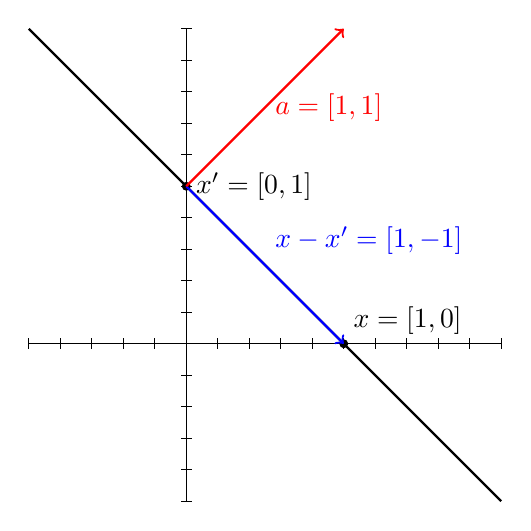
\begin{tikzpicture}[scale=2]
  %axis
  \draw (-1,0) -- coordinate (x axis mid) (2,0);
  \draw (0,-1) -- coordinate (y axis mid) (0,2);
  %ticks
  \foreach \x in {-1,-0.8,...,2}
    \draw (\x,1pt) -- (\x,-1pt);
  \foreach \y in {-1,-0.8,...,2}
  \draw (1pt,\y) -- (-1pt,\y);


  \draw[thick] (-1,2) -- (2,-1); 

  \fill (1,0) circle (.8pt) node [anchor=south west] {$x=[1,0]$};
  \fill (0,1) circle (.8pt) node [anchor=west] {$x'=[0,1]$};

  \draw[thick,->,blue] (0,1) -- node [anchor = south west] {$x-x'=[1,-1]$}  (1,0);
       
  \draw[thick,->,red] (0,1) -- node [anchor=west] {$a=[1,1]$} (1,2);

\end{tikzpicture}

\end{center}

\end{minipage}\hspace*{1cm}\begin{minipage}[t]{\textwidth-7cm}
  \vspace{0pt}
Ešte pripomeňme, že ak  sme v $m$-rozmernom priestore, nadrovina $\cal H$ je množina bodov \bm{x} spĺňajúcich
rovnosť $a_1x_1+\cdots+a_mx_m=1$ (jednotka na pravej strane je takmer všeobecná:
ľubovoľná nadrovina, ktorá neprechádza bodom $[0,\ldots,0]$ sa dá normovaním upraviť
na tento tvar). Ak označíme $\pair{\cdot}{\cdot}$ skalárny súčin, je
$\cal H$ definovaná ako $\pair{\bm{x}}{\bm{a}}=1$. 
Body, pre ktoré $\pair{\bm{x}}{\bm{a}}<1$ sú pod $\cal H$, a body
$\pair{\bm{x}}{\bm{a}}>1$ nad $\cal H$.
Vektor \bm{a} je {\em normálový vektor} $\cal H$ a pre ľubovoľné dva body \bm{x}, \bm{x'} z $\cal H$ platí,
$$\pair{\bm{x}-\bm{x'}}{\bm{a}}=\sum_{i=1}^m(x_i-x'_i)a_i=\pair{\bm{x}}{\bm{a}}-\pair{\bm{x'}}{\bm{a}}=0.$$

\noindent
V dvoch rozmeroch je nadrovinou priamka, tá na obrázku vľavo je daná rovnicou
$x_1+x_2=1$.

\end{minipage}

\noindent
Naše  úvahy o konvexných obaloch zavŕšime nasledovným pozorovaním, ktoré je
pre dva a tri rozmery úplne zjavné:

\begin{lema}
  \label{lm:KO:2}
  Majme body $\bm{x},\bm{a_1},\ldots,\bm{a_n}$ v $m$-rozmernom priestore. Nech $K$ je konvexný obal
  $\bm{a_1},\ldots,\bm{a_n}$. Potom platí:
  \begin{itemize}
    \item 
      Ak \bm{x} je vo vnútri\footnote{t.j. $K$ obsahuje \bm{x} aj nejaké jeho malé okolie} $K$,
      potom neexistuje nadrovina $\cal H$, ktorá prechádza cez \bm{x} a všetky body z $K$
      ležia na jednej strane $\cal H$.
    \item 
      Ak $\bm{x} \not\in K$,
      potom existuje nadrovina $\cal H$, ktorá prechádza cez \bm{x} a všetky body z $K$
      ležia na jednej strane $\cal H$.
  \end{itemize}
\end{lema}

\begin{dokaz}
  Prvá časť je ľahká: nech \bm{x} leží vo vnútri $K$ nech existuje taká nadrovina $\cal H$, že všetky body z $K$
  sú na jednej strane $\cal H$. Pretože $\bm{x}$ je vo vnútri $K$, existuje nejaký bod $\bm{x'}\in K$, ktorý leží
  na opačnej strane $\cal H$ ako všetky body z $K$, špeciálne ako body $\bm{a_i}$. 
  Lenže polpriestor ohraničený $\cal H$, ktorý obsahuje 
  všetky $\bm{a_i}$ je konvexné teleso, a preto z definície konvexného obalu $\bm{x'}\not\in K$.

\noindent
Ideme dokázať druhú časť.
Majme fixovaný  bod \bm{x} a pre body $\bm{y}\in K$ uvažujme euklidovskú vzdialenosť $f(\bm{y}):=||\bm{y}-\bm{x}||$. 
  Pretože $K$ je kompaktná množina a $f$ je spojitá funkcia nadobúdajúca kladné hodnoty, existuje bod
  $\bm{z}\in K$, na ktorom $f$ nadobúda minimum. Označme 
  \begin{align*}
    \bm{t}&=\bm{x}-\bm{z} & \kappa&= \pair{\bm{t}}{\bm{x}}
  \end{align*}

\begin{minipage}[t]{4.5cm}
  \vspace{0pt}
  \begin{myfig}{\textwidth}{svg/CHa}
  \end{myfig}
\end{minipage}\hspace*{1cm}\begin{minipage}[t]{\textwidth-7cm}
  \vspace{0pt}
  Nech $\cal H$ je nadrovina tvorená bodmi \bm{y}, pre ktoré $\pair{\bm{t}}{\bm{y}}=\kappa$.
  Zjavne $\bm{x}\in{\cal H}$. Platí
  $$0\le\sum_{i=1}^m(x_i-z_i)^2=%\sum_{i=1}^mx_i^2-2x_iz_i+z_i^2=
  \bpair{x}{x}-2\bpair{x}{z}-\bpair{z}{z}$$
  a preto
  \begin{align*}&\bpair{t}{z}=\pair{\bm{x}-\bm{z}}{\bm{z}}=\bpair{x}{z}-\bpair{z}{z}\le\\
                &\le\bpair{x}{x}-\bpair{x}{z}=\pair{\bm{x}-\bm{z}}{\bm{x}}=\bpair{t}{x}=\kappa
  \end{align*}
  \noindent
  Teraz stačí ukázať, že pre všetky body $\bm{y}\in K$ tiež platí $\bpair{t}{y}\le\kappa$, a teda
  ležia na rovnakej strane $\cal H$ ako \bm{z}.
\end{minipage}

\noindent
Majme teda $\bm{z}\in K$. 
Keďže \bm{z} minimalizuje vzdialenosť od \bm{x} a $K$ je konvexné teleso, pre všetky $0\le\lambda\le1$ platí
$||\bm{z}-\bm{x}||^2\le||(1-\lambda)\bm{z}+\lambda\bm{y}-\bm{x}||^2=
||(1-\lambda)(\bm{z}-\bm{x})+\lambda(\bm{y}-\bm{x})||^2$
a odtiaľ po priamočiarych úpravách
$0\le\lambda(\lambda-2)||\bm{z}-\bm{x}||^2+2\lambda(1-\lambda)\pair{\bm{z}-\bm{x}}{\bm{y}-\bm{x}}
+\lambda^2||\bm{y}-\bm{x}||^2
$.
Pretože $\lambda\ge0$, máme
$0\le(\lambda-2)||\bm{z}-\bm{x}||^2+2(1-\lambda)\pair{\bm{z}-\bm{x}}{\bm{y}-\bm{x}}
+\lambda||\bm{y}-\bm{x}||^2
$
a odtiaľ v limite pre $\lambda\mapsto0$
máme $0\le\pair{\bm{z}-\bm{x}}{\bm{y}-\bm{x}}-||\bm{z}-\bm{x}||^2
=\pair{\bm{z}-\bm{x}}{\bm{y}-\bm{x}}-\pair{\bm{z}-\bm{x}}{\bm{z}-\bm{x}}
=\pair{\bm{z}-\bm{x}}{\bm{y}}-\pair{\bm{z}-\bm{x}}{\bm{z}}=\bpair{t}{z}-\bpair{t}{y}
$.
Preto
$\bpair{t}{y}\le\bpair{t}{z}\le\kappa$, čo sme chceli dokázať.
\end{dokaz}

\end{shaded}

\noindent
Vráťme sa teraz k nášmu cieľu -- ukázať, že rovnaká hodnota
optimálneho riešenia v primárnej aj duálnej úlohe nie je náhoda. 
Pozrime sa na nasledovný príklad: Majme $m$-rozmerný priestor
$\R^m$ a v ňom $n$ bodov $\bm{a}_1,\ldots,\bm{a}_n$ (t.j. bod $\bm{a}_i$ má
súradnice $(a_{i1},a_{i2},\ldots,a_{im})$) a vektor $\bm{c}$. Cieľom je nájsť
čo najväčšie číslo $\alpha\in\R^+$ tak, že bod $\alpha\bm{c}$ leží v konvexnom
obale $K$ bodov $\bm{a}_1,\ldots,\bm{a}_n$. 

\begin{minipage}[t]{3.2cm}
  \vspace{0pt}
  \begin{myfig}{\textwidth}{svg/dualityCHa}
  \end{myfig}
\end{minipage}\hspace*{1cm}\begin{minipage}[t]{\textwidth-5cm}
  \vspace{0pt}
  \vskip 2ex
\noindent 
Predpokladajme pre jednoduchosť, že úloha má riešenie, t.j. polpriamka generovaná
vektorom \bm{c} pretína $K$. Z konvexity vyplýva, že prienik $K$ a polpriamky je úsečka.
Optimálne riešenie je preto bod $\alpha\bm{c}$, v ktorom polpriamka opúšťa $K$.
Podľa Lemy~\ref{lm:KO:1} sa 
body konvexného obalu sa dajú vyjadriť ako konvexná kombinácia bodov $\bm{a}_1,\ldots,\bm{a}_n$,
  t.j. náš hľadaný bod $\alpha\bm{c}$ sa musí dať napísať v tvare $z_1\bm{a}_1+\cdots+z_n\bm{a}_n$
  pre nejaké $z_1,\ldots,z_n\ge0$, kde $\sum_{i=1}^nz_i=1$. 
  Pre ľubovoľný prípustný bod
  $\alpha\bm{c}$ si označme  $y_j=\frac{z_j}{\alpha}$, potom
  platí 
\end{minipage}
  
  \begin{align*}
    y_j\ge&0 & \sum_{j=1}^ny_j=\frac{1}{\alpha} && \alpha\bm{c}=\alpha\sum_{j=1}^n\bm{a}_jy_j.
  \end{align*}
  Nájsť bod, pre ktorý je $\alpha$ maximálne, znamená nájsť bod, pre ktorý je $1/\alpha$ minimálne.
  Snažíme sa teda minimalizovať hodnotu $\sum_{j=1}^ny_j$ spomedzi takých $y_1,\ldots,y_n\ge 0$, 
\noindent
  pre ktoré $\sum_{j=1}^n\bm{a}_jy_j=\bm{c}$; stačí si uvedomiť, že z daných hodnôt \bm{y} vieme
  zrekonštruovať \bm{z} a $\alpha$.
Našu úlohu teda vieme zapísať ako úlohu lineárneho programovania:

\begin{equation}
  \label{eq:dualCHa}
\begin{array}{rrrrrcl}
  {\rm minimalizovať}     & y_1        & +\;y_2         & +\; \cdots  & +\;y_n   \\
  {\rm pri\ obmedzeniach} & a_{1,1}y_1 & +\;a_{2,1}y_2   & +\; \cdots  & +\;a_{n,1}y_n  & = & c_1 \\
                          & a_{1,2}y_1 & +\;a_{2,2}y_2   & +\; \cdots  & +\;a_{n,2}y_n  & = & c_2 \\
                          &   \vdots   &   \vdots       &   \ddots   &  \vdots      &  \vdots & \vdots\\ 
                          & a_{1,m}y_1 & +\; a_{2,m}y_2   & +\; \cdots  & +\;a_{n,m}y_n  & = & c_m \\
                          &\multicolumn{4}{r}{y_1,\ldots,y_n}&\ge&0
\end{array}
\end{equation}

\noindent
alebo skrátene
$$\text{(P)}\;\; \min_{\bm{y}\in\R^n}\left\{ \bm{1}\tr\bm{y} \mid A\tr\bm{y}=\bm{c},\;\bm{y}\ge\bm{0}\right\}, $$
kde $A$ je matica rozmerov $n\times m$, ktorej riadky sú tvorené súradnicami bodov $\bm{a}_1,\ldots,\bm{a}_n$.
Na program (\ref{eq:dualCHa}) použijeme náš dualizačný recept a dostaneme duálny program

\noindent
\begin{minipage}[t]{4cm}
  \vspace{0pt}
  \begin{myfig}{\textwidth}{svg/dualityCHb}
  \end{myfig}
\end{minipage}\hspace*{1cm}\begin{minipage}[t]{\textwidth-5cm}
  \vspace{0pt}

\begin{equation}
  \label{eq:dualCHb}
  \text{(D)}\;\;  \max_{\bm{x}\in\R^m}\left\{ \bm{c}\tr\bm{x} \mid A\bm{x}\le\bm{1}\right\}
\end{equation}

\noindent
Ako môžeme program (\ref{eq:dualCHb}) interpretovať? Zoberme si ľubovoľné prípustné riešenie \bm{x}. 
Nech ${\cal H}_{\bm{x}}$ je nadrovina daná bodmi \bm{y}, pre ktoré $\bpair{y}{x}=1$.
Obmedzenia programu (\ref{eq:dualCHb}) hovoria, že pre každý bod $\bm{a_i}$ je 
$\bpair{a_i}{x}\le1$, a z konvexity je preto celý konvexný obal $K$ pod ${\cal H}_{\bm{x}}$.
Ďalej ak označíme $\alpha=\frac{1}{\bm{c}\tr\bm{x}}$, tak  bod $\alpha\bm{c}$ leží v nadrovine 
${\cal H}_{\bm{x}}$, lebo $\pair{\alpha\bm{c}}{\bm{x}}=1$. Každému prípustnému riešeniu (\ref{eq:dualCHb})
teda zodpovedá bod $\alpha\bm{c}$ na polpriamke generovanej vektorom \bm{c}, ktorý (podľa Lemy~\ref{lm:KO:2})
neleží vo vnútri $K$.
Naviac je zrejmé, že optimálne riešenie je nezáporné, a preto môžme bez ujmy na všeobecnosti predpokladať,
že $\bpair{x}{c}=||\bm{x}||\cdot||\bm{c}||\cos\varphi\ge0$, kde $\varphi$ je uhol, ktorý zvierajú
vektory \bm{x} a \bm{c}. Preto nás zaujímajú iba tie prípustné riešenia, ktorým zodpovedajú
body $\alpha\bm{c}$ ležiace na polpriamke generovanej \bm{c} za $K$.
\end{minipage}

\vspace*{-4ex}
\noindent
Platí to aj naopak. Zoberme si hocijaký bod $\alpha\bm{c}$ ležiaci za $K$. Podľa Lemy~\ref{lm:KO:2}
existuje nadrovina $\cal H$ taká, že všetky body z $K$ ležia pod ňou. Nech $\cal H$ je tvorená
bodmi \bm{y} spĺňajúcimi $\bpair{x}{y}=1$ pre nejaký vektor \bm{x}, potom platí $A\bm{x}\le1$.
Zároveň, pretože $\cal H$ prechádza cez $\alpha\bm{c}$, platí 
$\pair{\bm{x}}{\alpha\bm{c}}=1=\alpha\bpair{x}{c}$, a teda $\alpha=\frac{1}{\bm{c}\tr\bm{x}}$.
Pre maximálnu hodnotu $\bm{c}\tr\bm{x}$ je príslušná $\alpha$ minimálna, a preto program (\ref{eq:dualCHb})
vyžaduje nájsť minimálne $\alpha$ tak, aby bol $\alpha\bm{c}$ ležal za $K$ na polpriamke generovanej 
vektorom \bm{c}. To je ale zjavne bod, v ktorom polpriamka opúšťa $K$, a teda programy
(\ref{eq:dualCHa}) a (\ref{eq:dualCHb}) majú rovnaké optimálne riešenie.
Dokázali sme teda tvrdenie

\begin{lema}
  \label{lm:strongdualityprep}
  Ak primárny program $\min_{\bm{y}\in\R^n}\left\{ \bm{1}\tr\bm{y} \mid A\tr\bm{y}=\bm{c},\;\bm{y}\ge\bm{0}\right\}$
má prípustné riešenie, potom aj duálny program 
$\max_{\bm{x}\in\R^m}\left\{ \bm{c}\tr\bm{x} \mid A\bm{x}\le\bm{1}\right\}$
má prípustné riešenie a optimálne hodnoty oboch programov sa rovnajú.
\end{lema}

\noindent
Keby sa nám podarilo Lemu~\ref{lm:strongdualityprep}
zovšeobecniť na programy tvaru  
$\min_{\bm{y}\in\R^n}\left\{ \bm{b}\tr\bm{y} \mid A\tr\bm{y}=\bm{c},\;\bm{y}\ge\bm{0}\right\}$
pre ľubovoľný vektor \bm{b},
boli by sme spokojní, lebo každý lineárny program sa dá napísať v takomto tvare. 
Majme teda primárny program
\begin{equation}
  \label{eq:dualgenP}
  \text{(P)}\;\; \min_{\bm{y}\in\R^n}\left\{ \bm{b}\tr\bm{y} \mid A\tr\bm{y}=\bm{c},\;\bm{y}\ge\bm{0}\right\}
\end{equation}
a k nemu duálny program
\begin{equation}
  \label{eq:dualgenD}
  \text{(D)}\;\;\max_{\bm{x}\in\R^m}\left\{ \bm{c}\tr\bm{x} \mid A\bm{x}\le\bm{b}\right\}\hspace*{10ex}
\end{equation}
\noindent
Uvažujme najprv vektory \bm{b} také, že všetky zložky $b_i>0$.
Označme 
\begin{align}
  \label{eq:dualgenNote1}
  \bm{a}_i'=&\frac{1}{b_i}\bm{a}_i & y_j'=&b_jy_j 
\end{align}

\noindent
Platí $\bm{b}\tr\bm{y}=\sum_{j=1}^nb_jy_j=\bm{1}\tr\bm{y}'$ a pre každé $i\in\{1,\ldots,m\}$
$\sum_{j=1}^ma_{ji}y_j=\sum_{j=1}^ma'_{ji}b_i\frac{y_j'}{b_j}$. Pretože $b_j>0$,  program (\ref{eq:dualgenP})
je ekvivalentný\footnote{v tom zmysle, že každému riešeniu programu (\ref{eq:dualgenP}) prislúcha nejaké riešenie 
programu (\ref{eq:dualgen3}) s rovnakou hodnotou a naopak}s programom
\begin{equation}
  \label{eq:dualgen3}
  \min_{\bm{y'}\in\R^n}\left\{ \bm{1}\tr\bm{y'} \mid A'\bm{y'}=\bm{c},\;\bm{y'}\ge\bm{0}\right\} 
\end{equation}
kde stĺpce matice  $A'$ sú vektory $\bm{a}_i'$.
Podľa Lemy~\ref{lm:strongdualityprep}, ak má program (\ref{eq:dualgen3}) prípustné riešenie, tak jeho optimum
je rovnaké ako optimum programu
\begin{equation}
  \label{eq:dualgen4}
  \max_{\bm{x'}\in\R^m}\left\{ \bm{c}\tr\bm{x'}\mid {A'}\tr\bm{x'}\le\bm{1}\right\}
 \end{equation}
 Obmedzenia programu (\ref{eq:dualgen4}) sú v tvare $\sum_{j=1}^ma_{ji}'x'_j\le1$ a tak s použitím
 označenia (\ref{eq:dualgenNote1}) dostávame, že programy (\ref{eq:dualgen4}) a (\ref{eq:dualgenD}) sú ekvivalentné,
 preto ak (\ref{eq:dualgenP}) má prípustné riešenie, má ho aj (\ref{eq:dualgenD}) a hodnoty optima sú rovnaké.

\begin{prob}
  Upravte predchádzajúci postup tak, aby platil pre $b_i\ge0$.
\end{prob}

\noindent
Nech teraz \bm{b} nadobúda ľubovoľné hodnoty a nech $\bm{\tilde{x}}$ je prípustné riešenie (\ref{eq:dualgenD}).
Označme 
\begin{align}
  \label{eq:dualgen5}
  \bm{x'}&=\bm{x}-\bm{\tilde{x}} & b_i'&=b_i-\bm{a}_i\tr\bm{\tilde{x}}
\end{align}

\noindent
Ako sa v tomto označení zmenia programy (\ref{eq:dualgenP}) a (\ref{eq:dualgenD})?
Pre prípustné riešenia \bm{x}, \bm{y} platí
$$
\begin{array}{ll}
  \bm{c}\tr\bm{x} &= \bm{c}\tr\bm{x'} + \bm{c}\tr\bm{\tilde{x}}\\
  \bm{b}\tr\bm{y} &= \sum_{i=1}^nb_iy_i = \sum_{i=1}^nb'_iy_i+\sum_{i=1}^ny_i(\bm{a}_i\tr\bm{\tilde{x}})=
  \bm{b'}\tr\bm{y}+\sum_{i=1}^ny_i\sum_{j=1}^ma_{i,j}\tilde{x}_j =\\
  &= \bm{b'}\tr\bm{y}+ \sum_{j=1}^m\tilde{x}_j(\sum_{i=1}^ny_ia_{i,j}) =
  \bm{b'}\tr\bm{y}+\bm{c}\tr\bm{\tilde{x}}
\end{array}
$$
kde posledná rovnosť vyplýva z toho, že $A\tr\bm{y}=\bm{c}$. 
Pretože $\bm{c}\tr\bm{\tilde{x}}$ je konštanta, programy  (\ref{eq:dualgenP}) a (\ref{eq:dualgenD}) vieme 
ekvivalentne zapísať ako
\begin{align*}
  (\text{P}')\;\; \min_{\bm{y}\in\R^n}\left\{ \bm{b'}\tr\bm{y} \mid A\tr\bm{y}=\bm{c},\;\bm{y}\ge\bm{0}\right\}
  &&
 (\text{D}')\;\; \max_{\bm{x'}\in\R^m}\left\{ \bm{c}\tr\bm{x'} \mid A\bm{x'}\le\bm{b'}\right\}
\end{align*}

\noindent
Navyše z prípustnosti $\bm{\tilde{x}}$ pre (\ref{eq:dualgenD}) vyplýva, že $\bm{b'}\ge\bm{0}$ a preto
môžeme aplikovať predchádzajúci prípad.

\noindent
Načrtli sme\footnote{pre kompletný dôkaz treba ošetriť ešte niekoľko 
špeciálnych prípadov, ktoré prenechávame na čitateľa} dôkaz fundamentálnej vety v teórii lineárneho programovania:

\begin{framed}
  \begin{veta}[Silná veta o dualite]
    \label{thm:strongduality}
    Pre dvojicu duálnych lineárnych programov
    \begin{align*}
      \text{(P)}\;\; \min_{\bm{y}\in\R^n}\left\{ \bm{b}\tr\bm{y} \mid A\tr\bm{y}=\bm{c},\;\bm{y}\ge\bm{0}\right\}
      &&
      \text{(D)}\;\;\max_{\bm{x}\in\R^m}\left\{ \bm{c}\tr\bm{x} \mid A\bm{x}\le\bm{b}\right\}\hspace*{10ex}
    \end{align*}
    Platí práve jedna zo štyroch možností:
    \begin{enumerate}
      \item (P) ani (D) nemajú žiadne prípustné riešenie
      \item (P) je neohraničený a (D) nemá prípustné riešenie
      \item (D) je neohraničený a (P) nemá prípustné riešenie
      \item (P) aj (D) majú prípustné riešenie. V tom prípade sa optimálne hodnoty (P) a (D) rovanjú.
    \end{enumerate}
  \end{veta}
\end{framed}

